\documentclass[10pt,a4paper]{article}
\usepackage[margin=17mm]{geometry}
\usepackage{graphicx,amsmath,booktabs,hyperref}
\setlength{\parindent}{0pt}\setlength{\parskip}{6pt}
\begin{document}
\begin{center}{\Large Target-density study and reoptimisation}\\[3pt]
Section 3.4 reconstruction of Stoddard et al. (2026)\\
\small DOI: \href{https://doi.org/10.20935/AcadDrug8407}{10.20935/AcadDrug8407}\end{center}
\textbf{Status: workflow reproduced; numerical validation remains unsuccessful.}
The authors' full model, physiological inputs and optimiser configuration are unavailable. These results use our existing ODE reconstruction and frozen calibration; they are not recovered author simulations. No parameters were fitted to Figures 7 or 8.

\textbf{What the paper did.} Figure 7 varies both tumour target densities independently, keeping the Figure 6 antibody fixed. Figure 8 uses one unequal-density pair and changes its binding rates. It does not reoptimise at every density-grid point. Supplementary Figure S4 extends the fixed-antibody sweep to lower densities.

\textbf{Matched settings.} Equal-density reference: $\rho_1=\rho_2=10^{-10}$ mol/dm$^2$, $k_{on,1}=k_{on,2}=10^4$ M$^{-1}$s$^{-1}$, $k_{off,1}=k_{off,2}=1$ s$^{-1}$. Unequal case: $\rho_1=10^{-9}$, $\rho_2=5\times10^{-11}$ mol/dm$^2$. Table 2 changes only $k_{on,2}$ to $5\times10^4$. These give $K_{D,1}=100$ and $K_{D,2}=20$ $\mu$M. The table therefore increases T2 affinity, although the narrative describes a reduction.

Dose: $4\times10^{-6}$ mol over 2 h; DAR: 1; payload EC$_{50}$: $4\,\mu$M; receptor turnover interpreted as $2$ h$^{-1}$. Score at 24 h, inferred from plotted traces. Healthy target density is always 25\% of the corresponding tumour density; tumour cell frequency 0.03\%, healthy T1-only 10\%, T2-only 10\%, dual-positive 1\%, neither 79\%. Literal published frequencies are used despite their 100.03\% sum.

\textbf{Frozen reconstruction assumptions.} Total cell burden $4.7263957\times10^{12}$ and intracellular volume $4.1329906\times10^{-13}$ L were calibrated previously to approximate Figure 4b and 6b tumour uptake (56 and 280 $\mu$M). Central/peripheral volumes: 11.3/41.5 L; intercompartmental flow: 1.05 L/h; clearance: 0.1 L/h; cell area: $5\times10^{-8}$ dm$^2$; membrane on-rates: $2.4\times10^{13}$ dm$^2$mol$^{-1}$s$^{-1}$. Adoption of these reference/inferred values by the authors is unconfirmed. Complexes share receptor turnover; no payload efflux, degradation or bystander killing. Changing target density does not change cell number or area.

\textbf{Endpoint comparison: our simulations, not digitised paper values.}
\begin{center}\small\begin{tabular}{lrrr}\toprule
Candidate & Tumour kill (\%) & Healthy kill (\%) & Uptake ($\mu$M)\\\midrule
Equal reference & 98.592 & 1.769 & 280.00 \\
Unequal: unchanged & 98.570 & 3.939 & 275.70 \\
Unequal: Table 2 & 98.567 & 4.589 & 275.05 \\
\bottomrule\end{tabular}\end{center}
The Table 2 candidate fails the stated $<1\%$ healthy-kill constraint in this reconstruction. Visually estimated Figure 8 endpoints are approximately 240 $\mu$M tumour uptake and 66\% T2 occupancy; our Table 2 simulation gives 275.05 $\mu$M and 82.21\%. These visual estimates are not exact validation data. The paper's healthy-kill curve also appears above 1\%, leaving an unresolved consistency question.
\newpage
\section*{Fixed-antibody density sweeps}
Each panel below uses 31 logarithmically spaced values per axis: 961 fresh ODE simulations. At every point, healthy densities are updated to $0.25\rho_1$ and $0.25\rho_2$; all rates and other inputs remain fixed. Black contours use the paper's levels where present. Circles mark the equal-density reference; triangles mark the unequal pair. No smoothing or fitted response surface is used.
\par
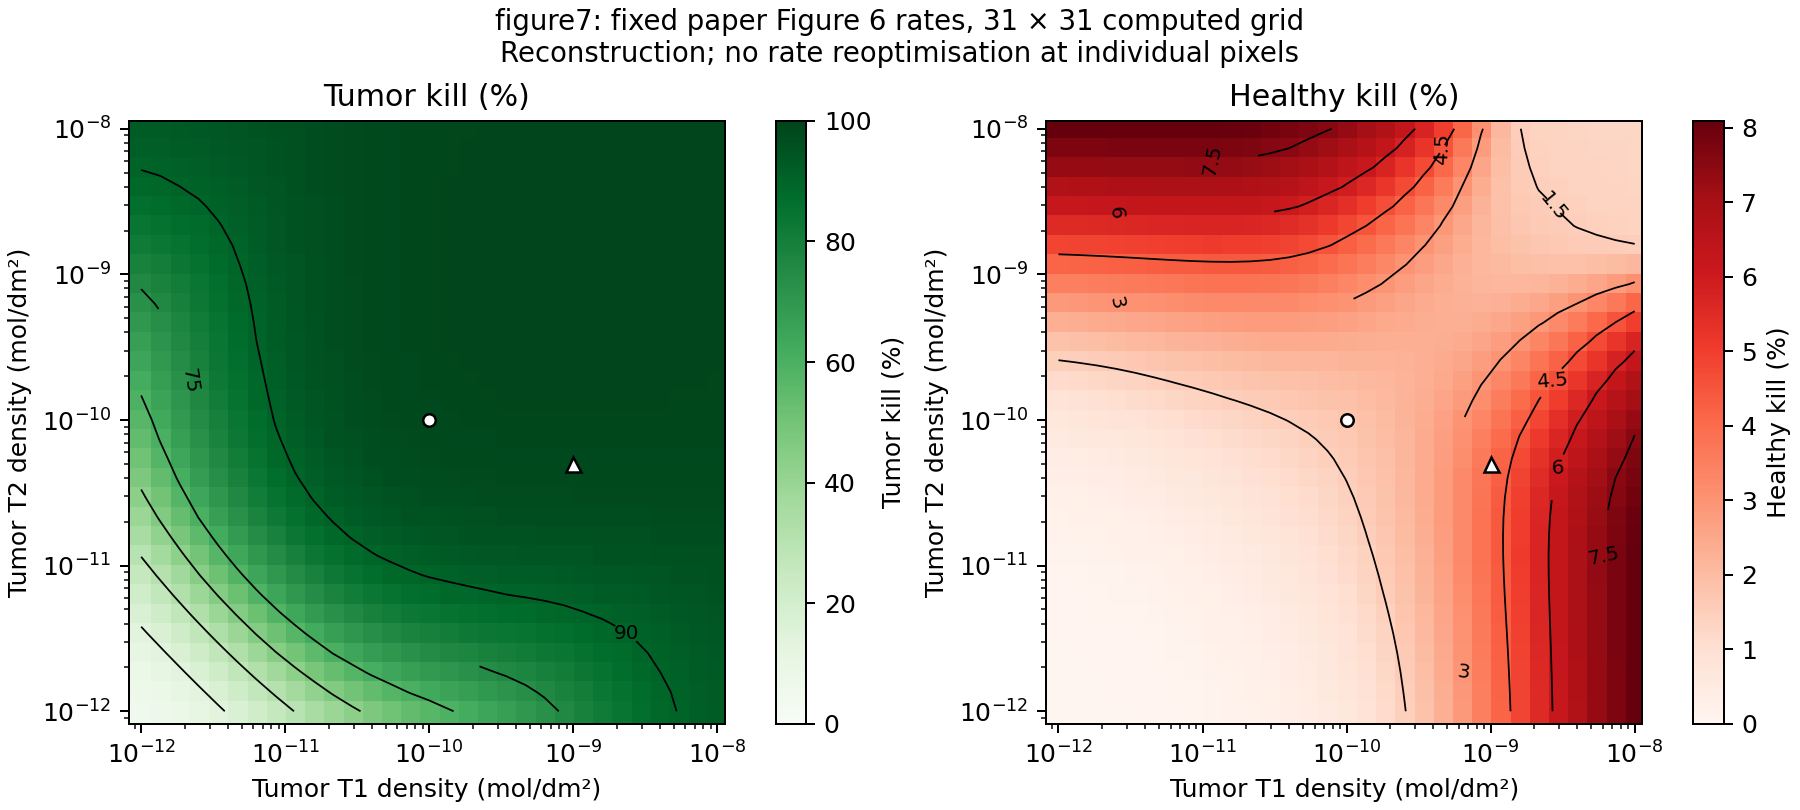
\includegraphics[width=\linewidth]{figure7.png}\par
\par
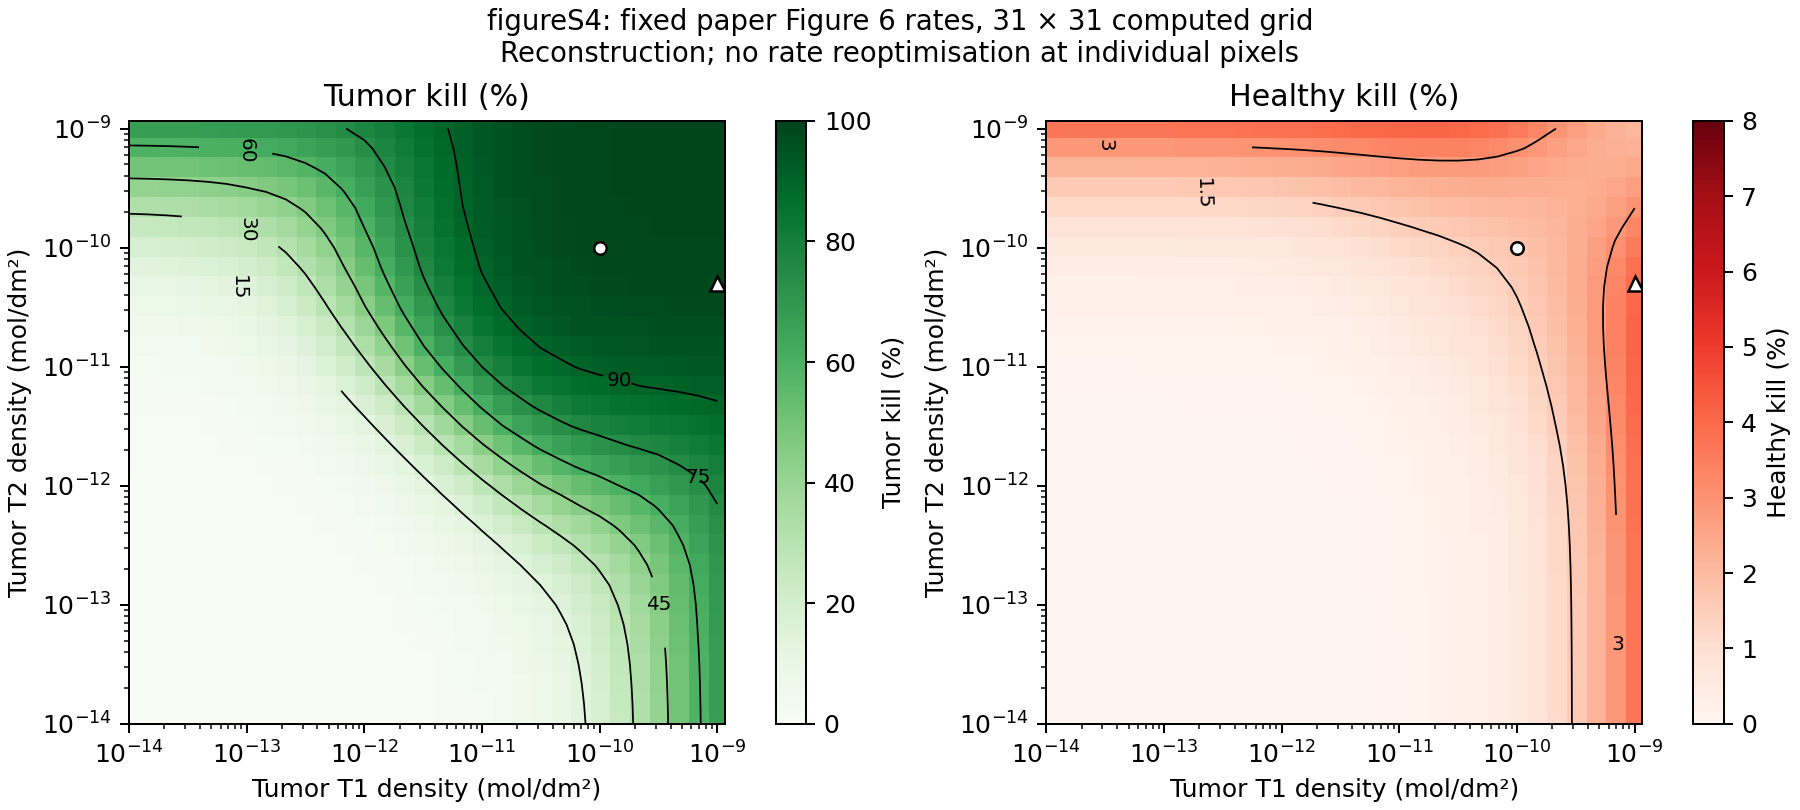
\includegraphics[width=\linewidth]{figureS4.png}\par
The contour patterns qualitatively resemble Figure 7: tumour kill rises with both densities, while unequal expression can raise healthy toxicity. At $(\rho_1,\rho_2)=(10^{-10},10^{-10})$, healthy kill is 1.77\%; changing only T2 to $10^{-9}$ raises it to 3.56\%. Thus a tenfold ratio is not a universal safety guarantee; absolute density matters. No quantitative contour-error metric has been established against digitised paper data. The colours show endpoint kill, not random-search candidates. Smooth contours reflect a structured density grid; visual smoothness alone does not establish agreement with the paper. CSV files preserve every computed point and nine explicit equal/tenfold-density comparisons.
\newpage
\section*{Unequal-density comparison and independent optimisation}
\par
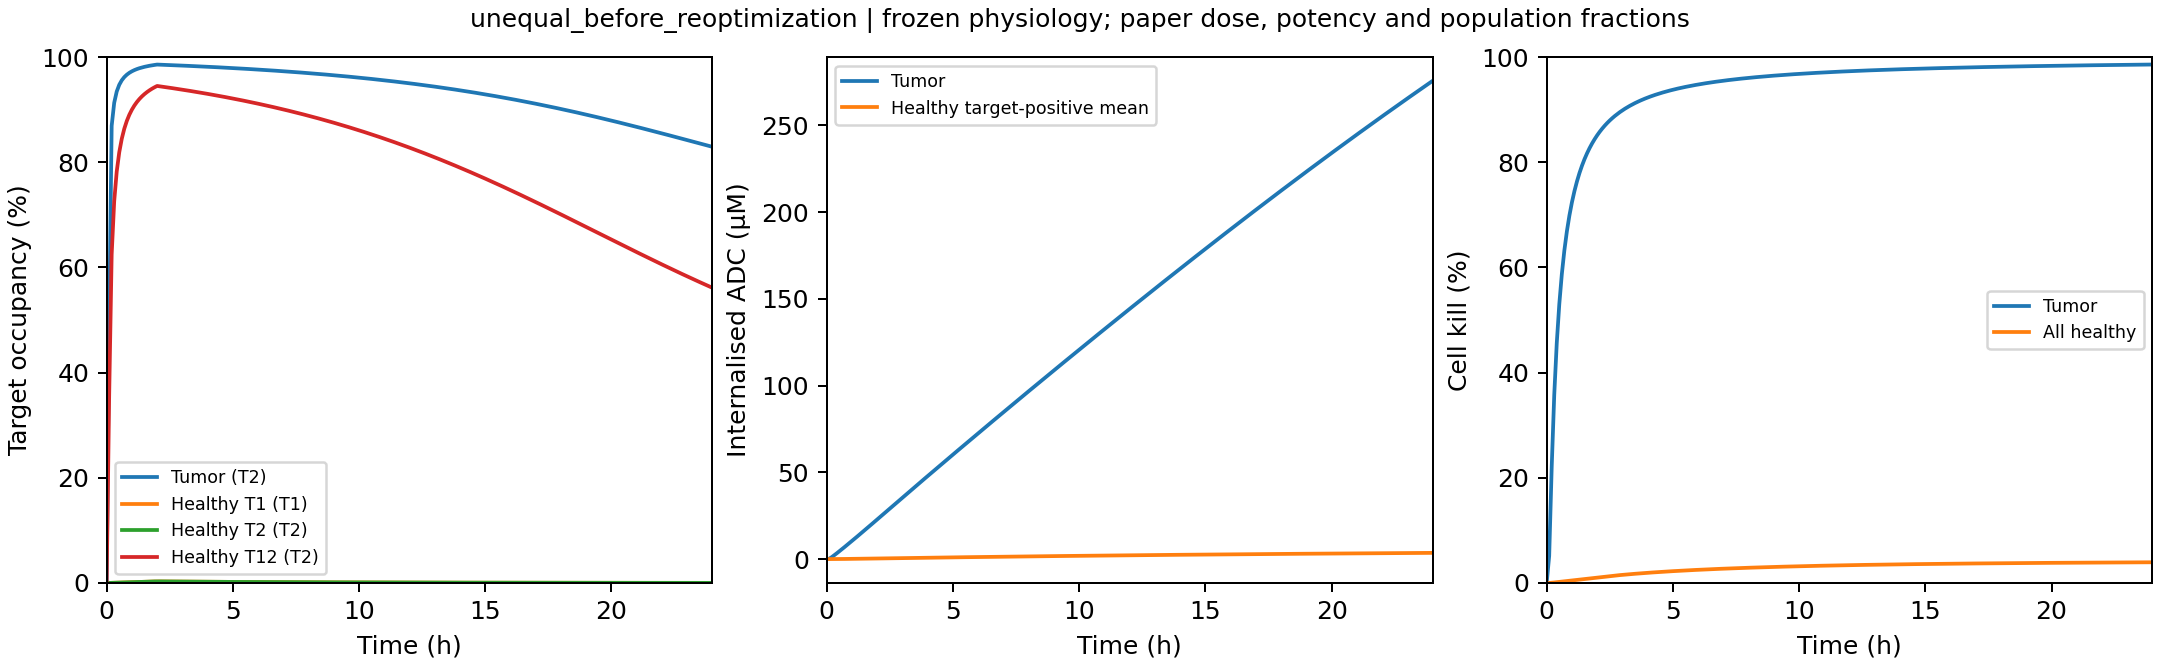
\includegraphics[width=\linewidth]{unequal_before_reoptimization.png}\par
\par
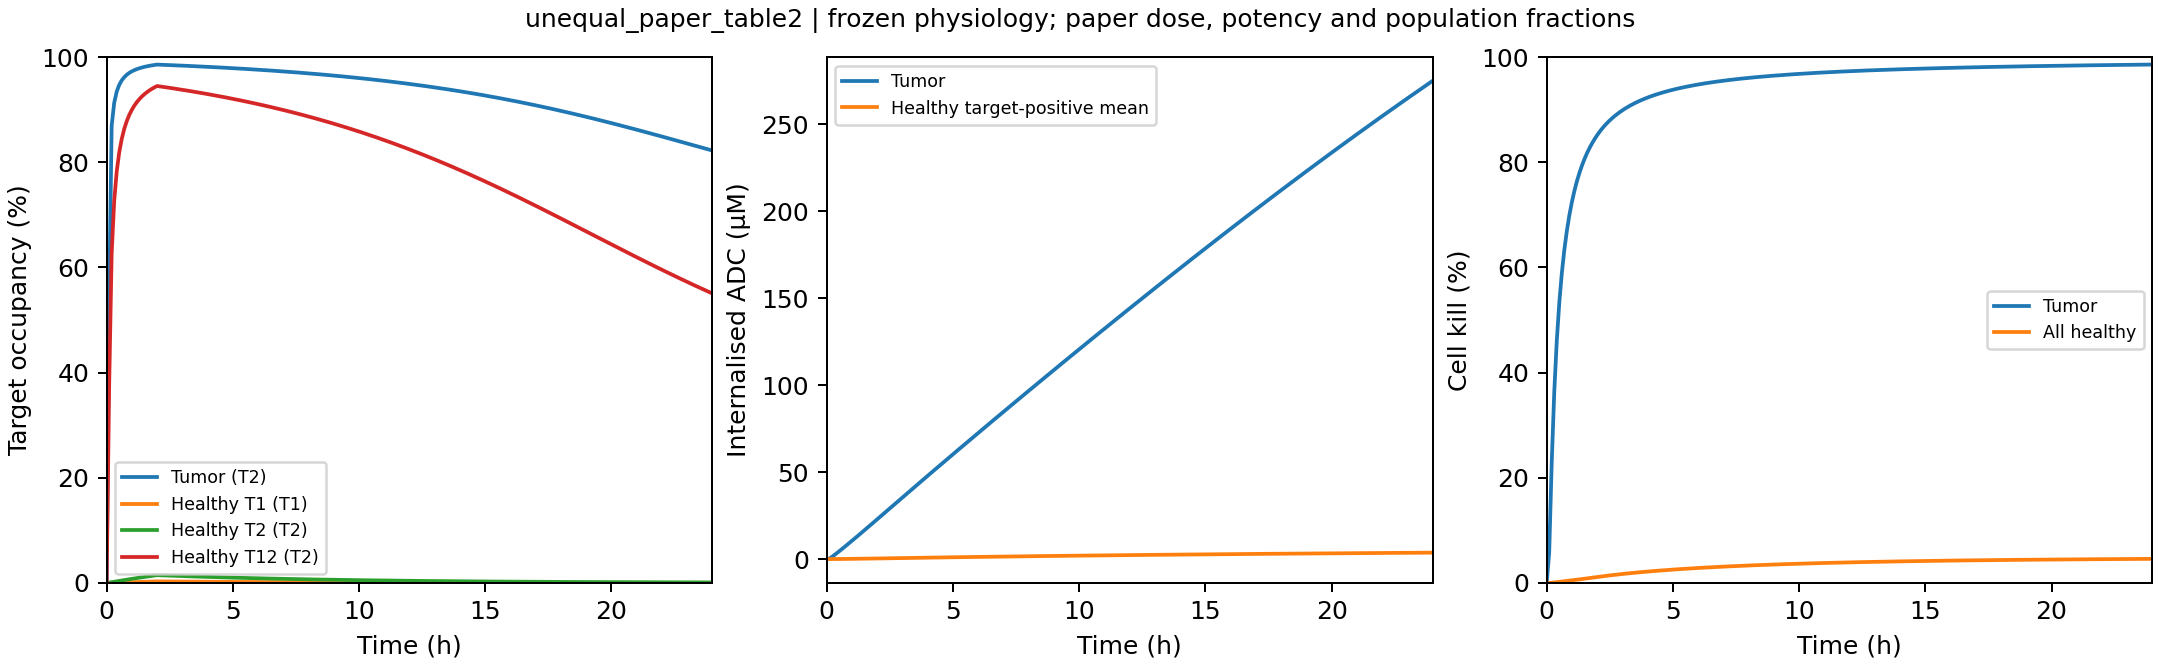
\includegraphics[width=\linewidth]{unequal_paper_table2.png}\par
Target occupancy is shown for T2 on tumour and dual-positive healthy cells, and each expressed target on single-positive healthy cells. Healthy uptake is the mean within target-positive healthy cells; healthy kill is averaged over all healthy cells. Averaging uptake before applying the nonlinear kill function would give an incorrect healthy-kill result.

\textbf{Independent search.} Four log-rate variables are varied, with $10^4\le k_{on,i}\le10^7$ M$^{-1}$s$^{-1}$ and $10^{-3}\le k_{off,i}\le1$ s$^{-1}$. These bounds are inferred from Figure 5 axes, not reported optimiser bounds. NSGA-II, population 48, two seeds (8407 and 2026), and 960 evaluations per seed are our implementation choices. All 16 rate-bound corners and the two published candidates seed each population. Objective and constraint:
\[
\min_{\theta=(\log_{10}k_{on,1},\log_{10}k_{off,1},\log_{10}k_{on,2},\log_{10}k_{off,2})}
\left(-E_T(24\mathrm{h}),E_H(24\mathrm{h})\right),\qquad E_H(24\mathrm{h})<0.01.
\]
The maximum tumour-kill feasible evaluation is selected and checked again with tighter solver tolerances. Healthy kill is a secondary Pareto objective; the paper specifies Platypus and efficacy maximisation with a toxicity constraint, but not its complete multiobjective formulation.

The searches evaluated 1889 candidates across two seeds. No feasible candidate was found; the lowest observed healthy kill was 3.939\%. This is finite-search evidence, not a proof of infeasibility.
\newpage
\section*{Exact computational chain in this reconstruction}
For each population $j$, free receptors $R_{1j},R_{2j}$, singly-bound ADC $B_{1j},B_{2j}$ and doubly-bound ADC $D_j$ have surface-density units. $C_c,C_p$ are free ADC concentrations; $A_j$ is intracellular payload concentration. Define
\begin{align*}
K_{D,i}&=k_{off,i}/k_{on,i},\\
v_{ij}&=k_{on,i} C_cR_{ij}-k_{off,i}B_{ij},\\
w_{1j}&=k_{2D,1}B_{2j}R_{1j}-q_1D_j,\quad
w_{2j}=k_{2D,2}B_{1j}R_{2j}-q_2D_j,\\
q_2&=k_{off,2},\qquad q_1=\frac{k_{off,1}k_{on,2}k_{2D,2}}{k_{on,1}k_{2D,1}}.
\end{align*}
The $q_1$ closure enforces detailed balance using the adopted Sengers convention; its use by the paper is unconfirmed. Increasing $k_{on,2}$ also changes $q_1$ under this closure, a material uncertainty for unequal-rate comparisons. With turnover $k=2/3600$ s$^{-1}$,
\begin{align*}
\dot R_{1j}&=k(\rho_{1j}-R_{1j})-v_{1j}-w_{1j},&
\dot R_{2j}&=k(\rho_{2j}-R_{2j})-v_{2j}-w_{2j},\\
\dot B_{1j}&=v_{1j}-w_{2j}-kB_{1j},&
\dot B_{2j}&=v_{2j}-w_{1j}-kB_{2j},\\
\dot D_j&=w_{1j}+w_{2j}-kD_j,&
\dot A_j&=\frac{a}{V_{cell}}k(B_{1j}+B_{2j}+D_j),\\
V_c\dot C_c&=u(t)-CL C_c-Q(C_c-C_p)-\sum_jN_ja(v_{1j}+v_{2j}),\\
V_p\dot C_p&=Q(C_c-C_p).
\end{align*}
Here $a$ is cell area, $N_j$ is population cell count, $Q$ is intercompartmental flow, $CL$ is clearance, and $u(t)=\mathrm{dose}/7200$ for the first 7200 seconds and zero thereafter. Flow and clearance are converted to litres per second. Initially $R_{ij}=\rho_{ij}$ and all other states are zero. A separate cumulative eliminated-dose state closes the drug mass balance.
\[
RO_{ij}=\frac{B_{ij}+D_j}{\rho_{ij}},\qquad
E_j=\frac{A_j}{EC_{50}+A_j},\qquad
E_T=E_{tumour},\qquad E_H=0.1E_{H1}+0.1E_{H2}+0.01E_{H12}.
\]
Occupancy is reported only for expressed targets. Zero-target healthy cells contribute zero kill. Percentages equal $100E$. These are instantaneous concentration-response estimates, not a separate cell-death ODE. Every search evaluation solves the complete time-dependent system; $K_D$ alone cannot determine the objective.

\textbf{Numerical checks.} BDF and Radau at tighter tolerances agree across the three fixed candidates and four Figure 7 grid corners. Maximum endpoint difference (fraction): 2.85e-10; maximum relative drug-mass error: 2.22e-14. Both density maps pass target-exchange symmetry checks. Numerical consistency supports the implementation, but does not validate its unpublished physiological assumptions.

\textbf{Reproduce.} From the repository, run \texttt{python replication/density\_study.py --grid 31 --nfe 960}, then \texttt{python replication/report\_density\_study.py}. Full inputs, candidate evaluations, grid data, trajectories and verification results are stored alongside this report. Exact reproduction still requires the authors' full ODEs, physiology, bound-state dissociation convention, optimisation bounds and objective implementation.
\end{document}
